\ppageno=15
\ppreviouspageno=14
\plineno=39
\psublineno=1

\newParkoszpage

{\relsize{-1}
\url{http://wbl.klf.uw.edu.pl/13/2/iParkosz.djvu?djvuopts=&page=55&zoom=width&showposition=0.5,0.18}

\url{http://wbl.klf.uw.edu.pl/13/2/iParkosz.djvu?djvuopts=&page=78&zoom=width&showposition=0.5,0.81}
}

\bigskip

\obeylines
\mono



\fullpreviouslines


{
\color{blue}

Tamen

eciam in suis locis possemus singulas predictas
}

\plineno=0

\fulllines

litteras seu earum exempla ponere, sicut et ponemus. Non

est enim vicium idem pluries repetere ex causa notandum.

% \def\splitlines{\advance\plineno by 1\psublineno=0\everypar{\advance\psublineno by 1\llap{\textcolor{green}{\the\ppageno-\ifnum\plineno<10 0\fi\the \plineno-\the\psublineno \ }}}}

% \def\newsplitline{\advance\plineno by 1}

\def\splitverse{\advance\plineno by 1\psublineno=0\everypar{\advance\psublineno by 1\llap{\textcolor{green}{\the\ppageno-\ifnum\plineno<10 0\fi\the \plineno-\the\psublineno \ }}\hskip5em}}

% nie działa licznik wierszy?
\def\fullverselines{\everypar{\advance\plineno by 1\llap{\the\ppageno-\ifnum\plineno<10 0\fi\the \plineno \hskip 1.5em}\hskip5em}}


\def\newverse{\advance\plineno by 1\psublineno=0\hskip10em}
\def\newversesubline{\hskip\indentV}
\def\newverseline{\advance\plineno by 1\psublineno=0}
\newdimen\indentV
\indentV=10em
%\setlength{\indentV}{10em}
\def\indentVerse{\hskip\indentV{}}

% MUFI SHORT VIRGULA
% skomentowac w artykule!

{

\catcode`\/=13
\def/{{\fontCardo }}

% 
\includegraphics[width=\hsize]{wierszP1m}

\splitverse

\parkosz{Ktho} \parkosz{chce} \parkosz{piſſaç} \parkosz{doſkoɲaɬe}

\indentVerse \parkosz{Ġøzik} \parkosz{poɬſki}

% 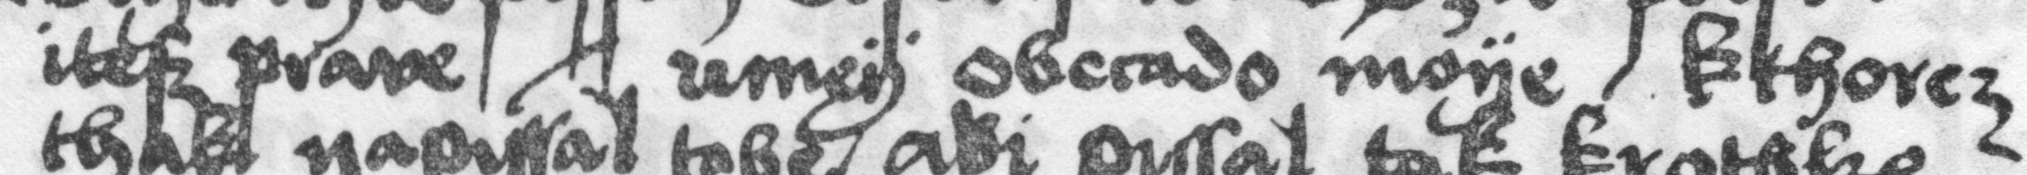
\includegraphics[width=\hsize]{wierszP2}

%\newverse
\splitverse

\parkosz{itefz} \parkosz{prave}/

\settowidth{\indentV}{\parkosz{itefz} \parkosz{prave}/}
\indentVerse \parkosz{uṃeij} \parkosz{obecado} \parkosz{ṃoije}/

% http://en.wikipedia.org/wiki/Ezh
% 'LATIN SMALL LETTER EZH' (U+0292)
	

\catcode `\^^M=5
\newtip{85}{Tak w rkp., z pewnością należy czytać \textit{ktorem}, a nie \textit{któreż}, co jednak
nie jest o tyle pewne, że w wyrazach, polskich w traktacie skrótów nie ma.}
\obeylines
\settowidth{\indentV}{\parkosz{itefz} \parkosz{prave}/ \parkosz{uṃeij} \parkosz{obecado} \parkosz{ṃoije}/}
\indentVerse \parkosz{kthore\conf{ʒ}{}}¹

% 85 Tak w rkp., z pewnością należy czytać Morem, a nie któreś, Co jednak

% nie jest o tyle pewne, że w wyrazach, polskich w traktacie skrótów nie ma.

% 
\includegraphics[width=\hsize]{wierszP3}


\splitverse

\parkosz{thak} \parkosz{ɲapiſſaḷ} \parkosz{toɓe}/

\settowidth{\indentV}{\parkosz{thak} \parkosz{ɲapiſſaḷ} \parkosz{toɓe}/}
\indentVerse  \parkosz{aɓi} \parkosz{piſſaḷ} \parkosz{tak} \parkosz{krothke}

% 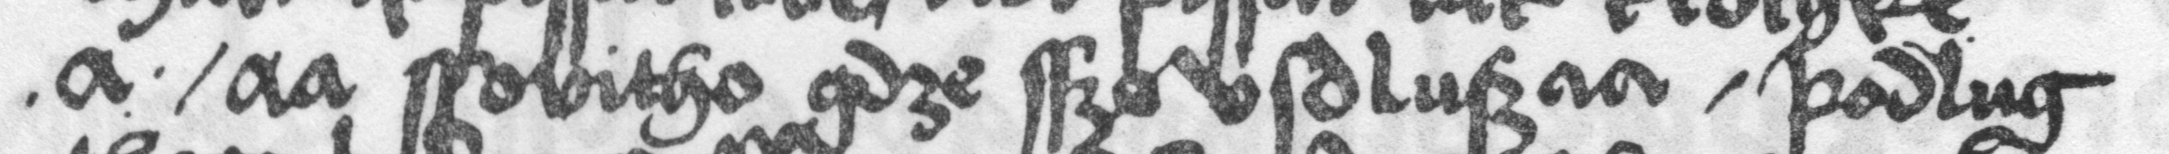
\includegraphics[width=\hsize]{wierszP4}

\splitverse

· \parkosz{a} ·/


\settowidth{\indentV}{· \parkosz{a} ·/}
%\def\indentVerse
% doesn't work:!
% \phantom{· \parkosz{a} ·/}
\indentVerse \parkosz{\textit{aa}} \parkosz{ſſovitho} \parkosz{ꝿdze} \parkosz{ſſzø} \parkosz{ʋſdḷuſzaa}/

\settowidth{\indentV}{· \parkosz{a} ·/ \parkosz{\textit{aa}} \parkosz{ſſovitho} \parkosz{ꝿdze} \parkosz{ſſzø} \parkosz{ʋſdḷuſzaa}/}
\indentVerse  \parkosz{podḷuꝿ}

% 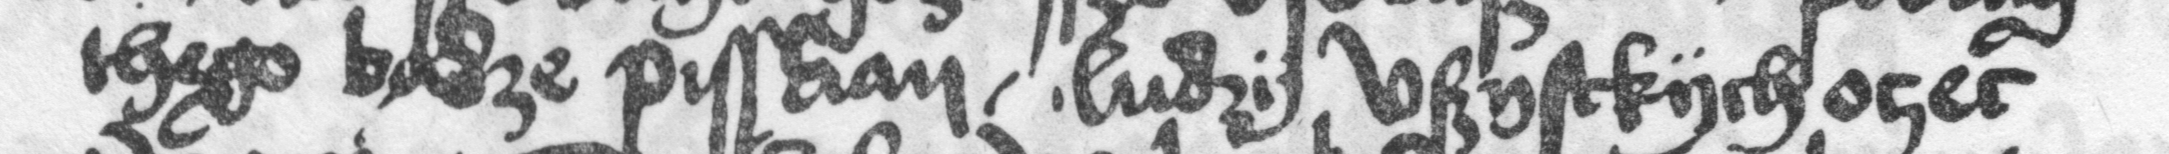
\includegraphics[width=\hsize]{wierszP5}

\splitverse

\parkosz{theꝿo} \parkosz{bødze} \parkosz{piſſaaɲ}/

% znika e!!!
\settowidth{\indentV}{\parkosz{theꝿo} \parkosz{bødze} \parkosz{piſſaaɲ}/}
\indentVerse \parkosz{ɬudzij} \parkosz{ʋſzyſtkijch} \parkosz{oçec}

% 
\includegraphics[width=\hsize]{wierszP6}

\splitverse

\parkosz{\textit{adaaɱ}}/

\settowidth{\indentV}{\parkosz{\textit{adaaɱ}}/}
\indentVerse \parkosz{A} \parkosz{theſz ġdze} · \parkosz{ƀ} · \parkosz{bødze} \parkosz{ġruube}/

% \newverseline

% 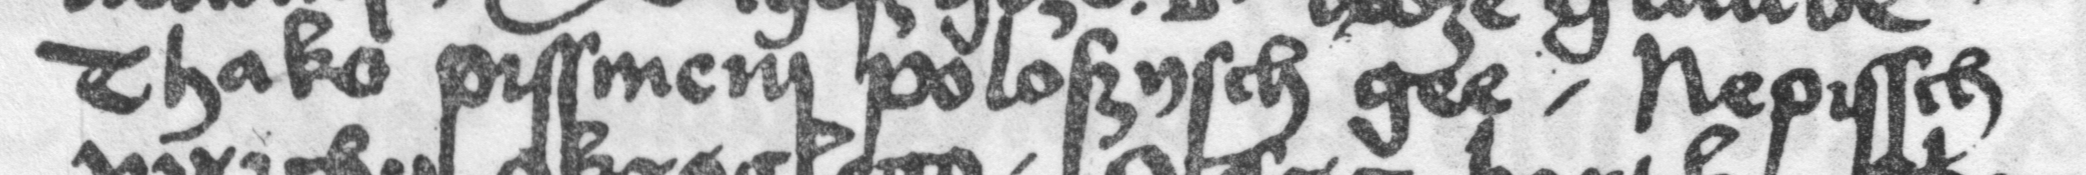
\includegraphics[width=\hsize]{wierszP7}

\splitverse

\parkosz{Thako} \parkosz{piſſṃeɱ} \parkosz{poḷoſzyſch} \parkosz{ġee}/

\settowidth{\indentV}{\parkosz{Thako} \parkosz{piſſṃeɱ} \parkosz{poḷoſzyſch} \parkosz{ġee}/}
\newversesubline \parkosz{Ṇepiſſch}

% 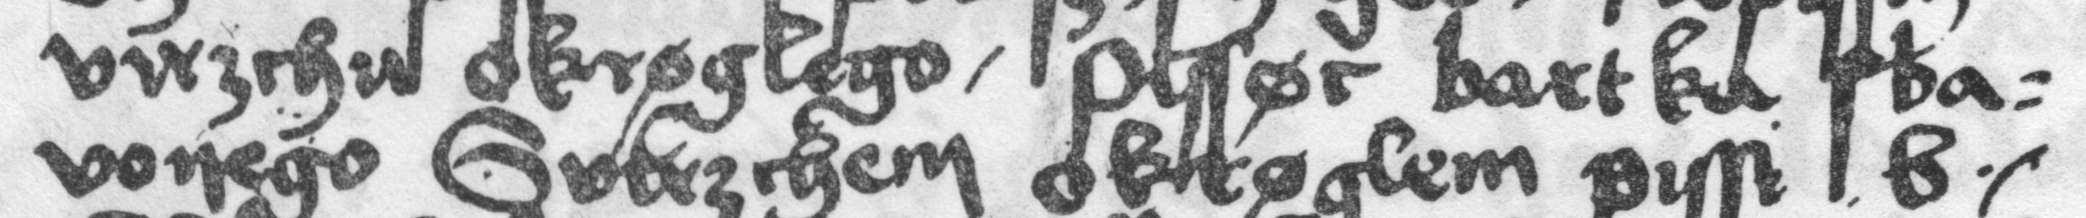
\includegraphics[width=\hsize]{wierszP8}

\splitverse \parkosz{virzchu} \parkosz{okrøꝿɬeꝿo}/

% hyphen!!!
\settowidth{\indentV}{\parkosz{virzchu} \parkosz{okrøꝿɬeꝿo}/}
\newversesubline \parkosz{Piſſøc} \parkosz{\textit{bartka}} \parkosz{\textit{\hyphh{ſba}{voɲeġo}}}

% 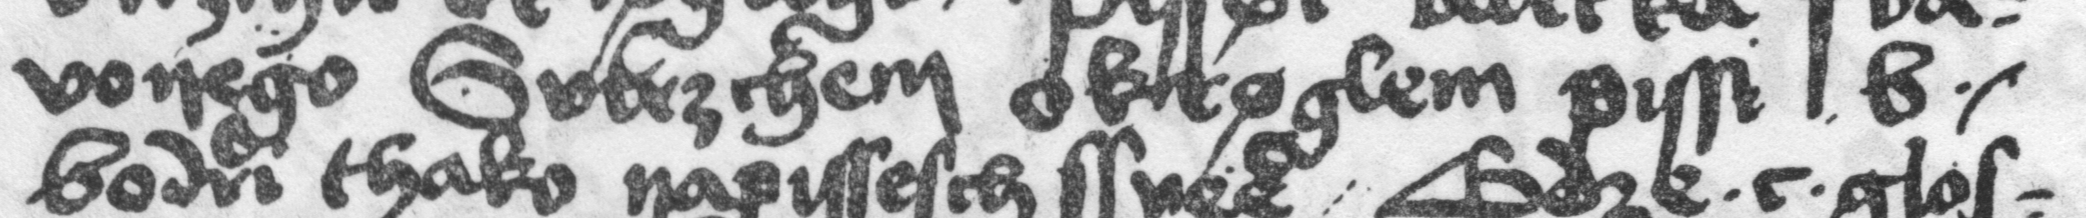
\includegraphics[width=\hsize]{wierszP9}

%\newverseline
\fullverselines

 \parkosz{\textit{\hypht{ſba}{voɲeġo}}} \parkosz{Svirzcheɱ} \parkosz{okrøꝿɬeṃ} \parkosz{piſſi} · \parkosz{ɓ} ·/

% 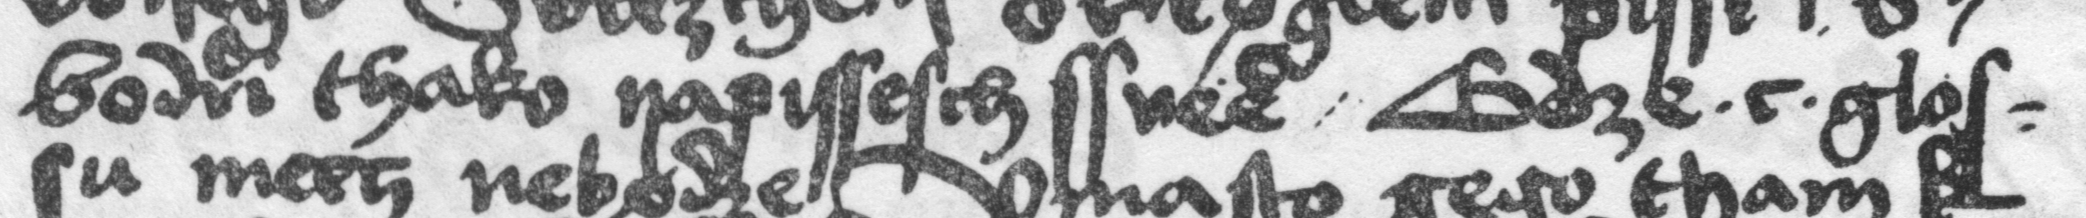
\includegraphics[width=\hsize]{wierszP10}

\plineno=11
\splitverse

\parkosz{\textit{ɓodri}} \parkosz{thako} \parkosz{ɲapiſſeſch} \parkosz{ſſvee}/

% zły numer!

\settowidth{\indentV}{\parkosz{\textit{ɓodri}} \parkosz{thako} \parkosz{ɲapiſſeſch} \parkosz{ſſvee}/}
\indentVerse \parkosz{Ġdze} · \parkosz{\textit{c}} · \parkosz{\hyphh{ġḷoſ}{ſu}}

% 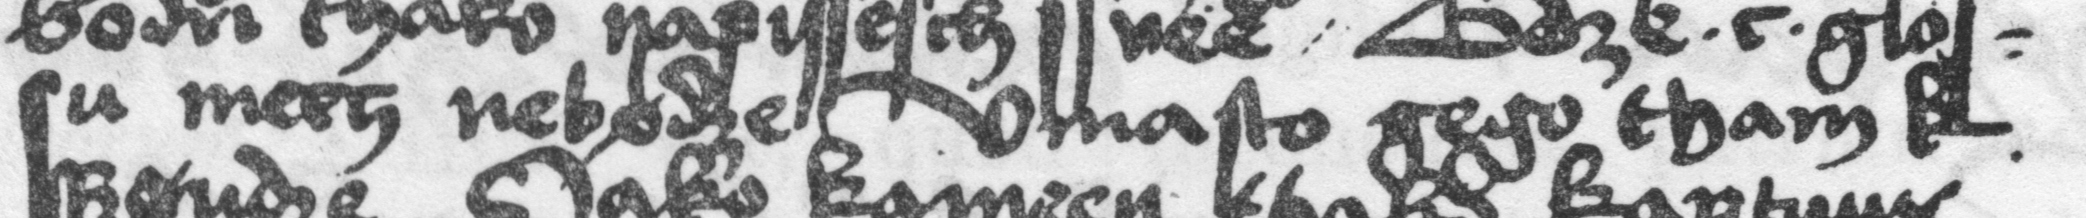
\includegraphics[width=\hsize]{wierszP11}

\splitverse

\parkosz{\hypht{ġḷoſ}{ſu}} \parkosz{ṃeeç} \parkosz{ṇebødze}

\settowidth{\indentV}{\parkosz{\hypht{ġḷoſ}{ſu}} \parkosz{ṃeeç} \parkosz{ṇebødze}}
\indentVerse \parkosz{Vṃaſto} \parkosz{ġeꝿo} \parkosz{thaṃ} \parkosz{\textit{k}}

% 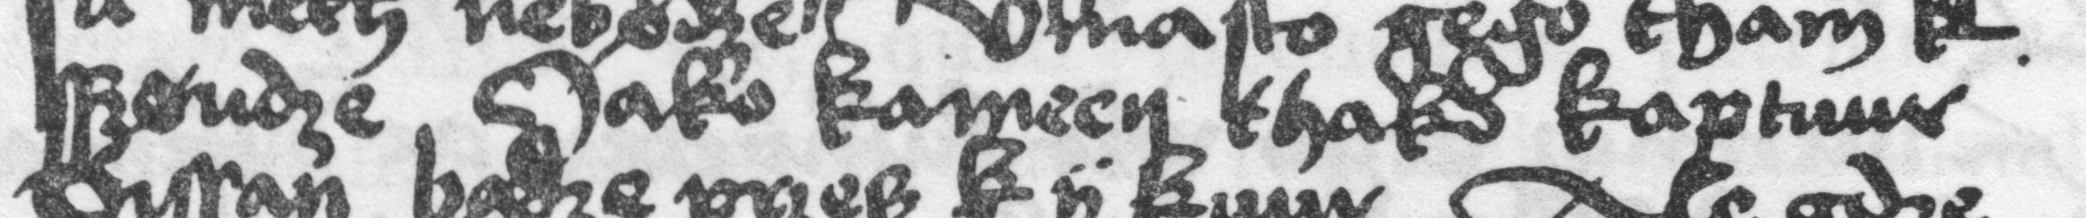
\includegraphics[width=\hsize]{wierszP12}

\splitverse

\parkosz{ſſzøṇdze}

\settowidth{\indentV}{\parkosz{ſſzøṇdze}}
\indentVerse \parkosz{Iako} \parkosz{\textit{kaṃeeɲ}} \parkosz{thako} \parkosz{\textit{kaᵽtuur}}

\newpage
% 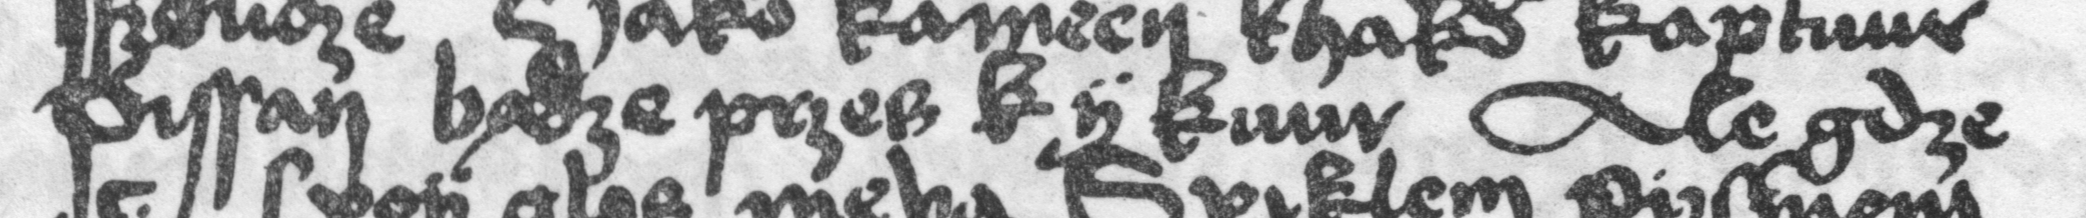
\includegraphics[width=\hsize]{wierszP13}

\splitverse

% brak Ƥ
\parkosz{Ƥiſſaɲ} \parkosz{bⱥdze} \parkosz{przes} \parkosz{\textit{k}} \parkosz{ij} \parkosz{\textit{kuur}}

\indentVerse \parkosz{Aɬe} \parkosz{ꝿdze}

% 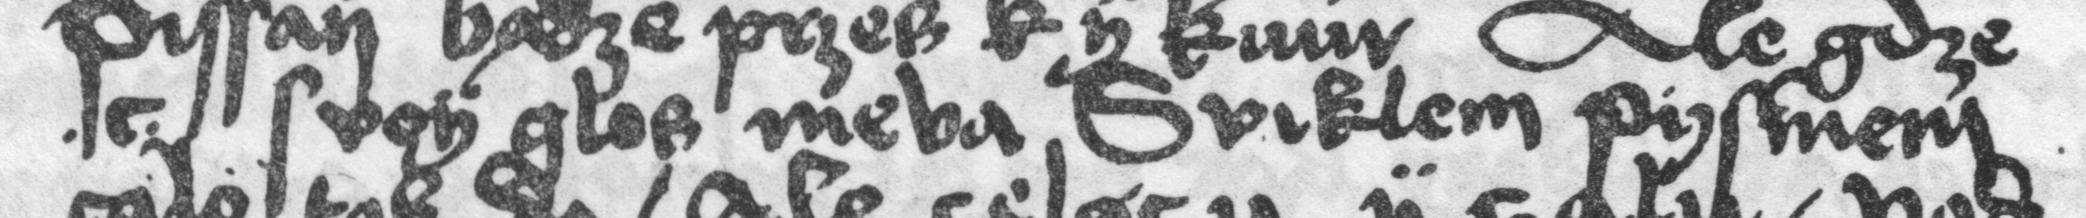
\includegraphics[width=\hsize]{wierszP14}

\splitverse

· \parkosz{\textit{c}} · \parkosz{ſvoij} \parkosz{ꝿḷos} \parkosz{ṃeʋa}

\indentVerse \parkosz{Svikḷeṃ} \parkosz{pijſṃeɱ}

% 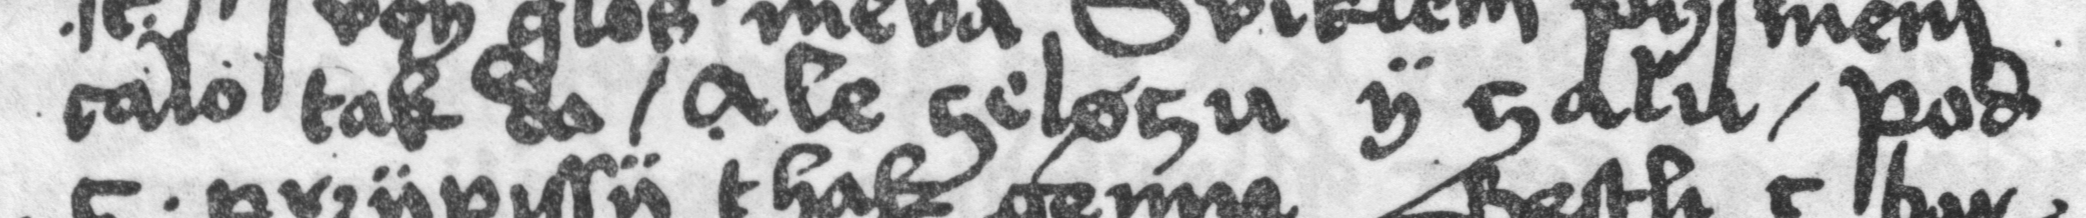
\includegraphics[width=\hsize]{wierszP15}

\splitverse

\parkosz{caḷo} \parkosz{tak} \parkosz{da}/

\indentVerse \parkosz{Aɬe} \parkosz{\textit{çeløçu}} \parkosz{ij} \parkosz{\textit{çalu}}/

\indentVerse  \parkosz{pod}

% 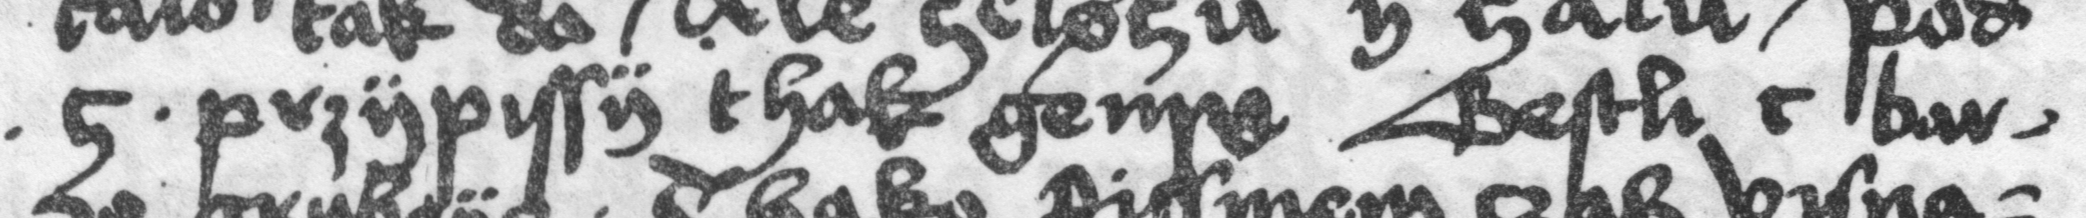
\includegraphics[width=\hsize]{wierszP16}

\splitverse

  · \parkosz{Q} · \parkosz{przijpiſſy} \parkosz{thak} \parkosz{ġeɱv}

\indentVerse \parkosz{Ġeſtɬi} \parkosz{\textit{c}} \parkosz{\hyphh{bar}{zo}}

% 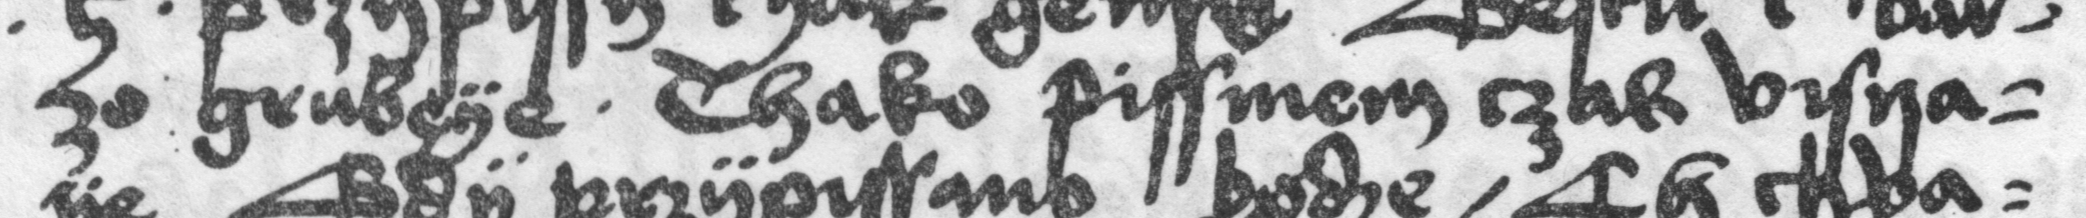
\includegraphics[width=\hsize]{wierszP17}

\newverseline \parkosz{\hypht{bar}{zo}} \parkosz{ġruɓeije}.

\indentVerse \parkosz{Thako} \parkosz{piſſṃeṃ} \parkosz{\textit{czas}} \parkosz{\hyphh{ʋiſɲa}{ije}}

% 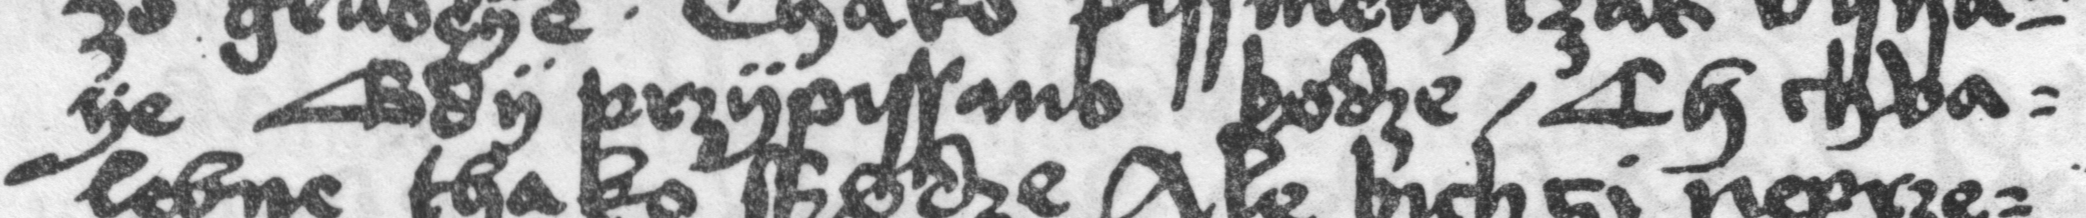
\includegraphics[width=\hsize]{wierszP18}

\newverseline \parkosz{\hypht{ʋiſɲa}{ije}} \parkosz{Ġdy} \add{h} \parkosz{przijpiſſaṇo} \parkosz{bødze}/

\indentVerse \parkosz{\textit{Ch}}  \parkosz{\hyphh{chʋa}{ɬebɲe}}

\newpage

% 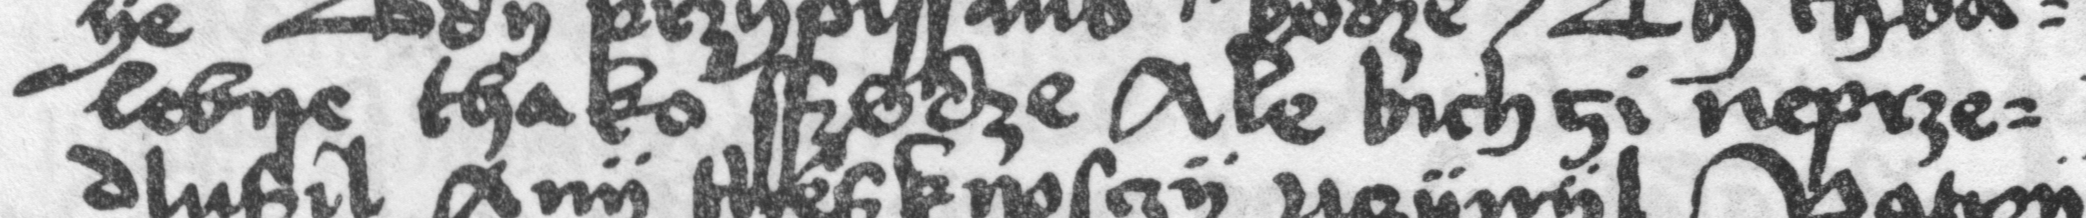
\includegraphics[width=\hsize]{wierszP19}

\splitverse

\parkosz{\hypht{chʋa}{ɬebɲe}} \parkosz{thako} \parkosz{ſſzødze}

\indentVerse \parkosz{Aɬe} \parkosz{bich} \parkosz{çi} \parkosz{\hyphh{ṇeprze}{dḷuſziḷ}}

% 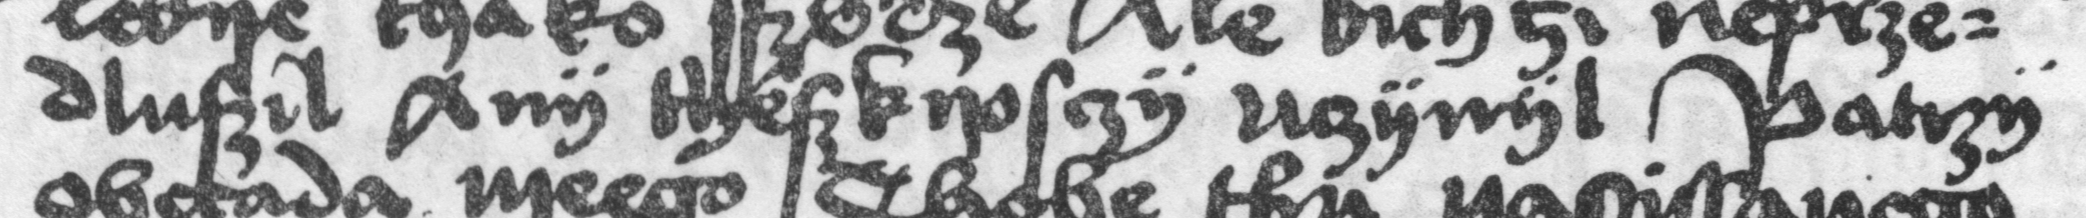
\includegraphics[width=\hsize]{wierszP20}

\splitverse

\parkosz{\hypht{ṇeprze}{dḷuſziḷ}}

\indentVerse \parkosz{Aṇij} \parkosz{theſzkɲoſczij} \parkosz{uczijṇijḷ}

\indentVerse \parkosz{Patrzij}

% 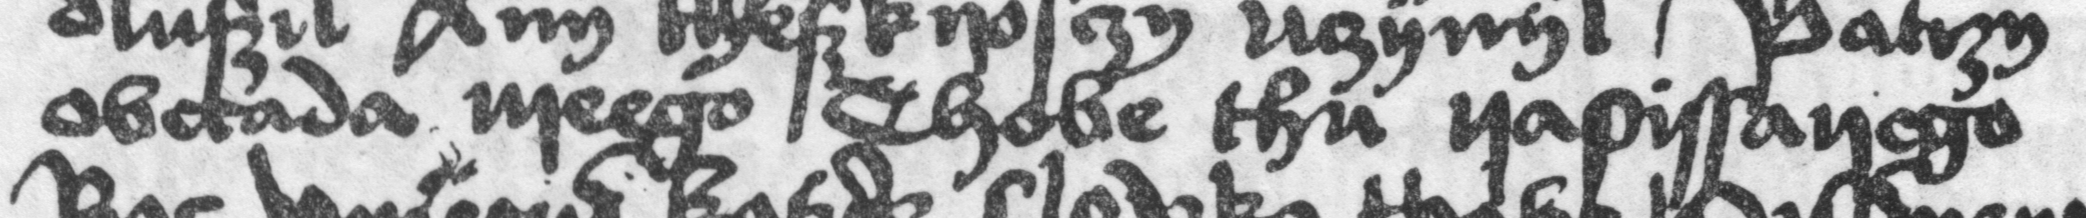
\includegraphics[width=\hsize]{wierszP21}

\splitverse

\parkosz{obecada} \parkosz{ɱeeġo}

\indentVerse \parkosz{Thoɓe} \parkosz{thu} \parkosz{ɲapiſſaɲeġo}

% 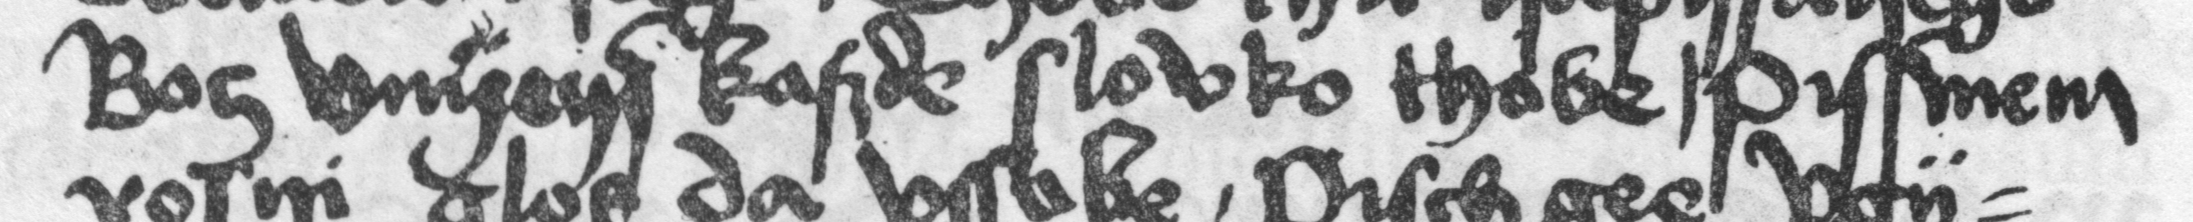
\includegraphics[width=\hsize]{wierszP22}

\splitverse

\parkosz{Boç} \parkosz{ʋṇye\conf{ɱ}{}} \parkosz{kaſzde} \parkosz{ſḷoʋko} \parkosz{thobe} /

\indentVerse \parkosz{Ƥiſſṃeɱ}

% 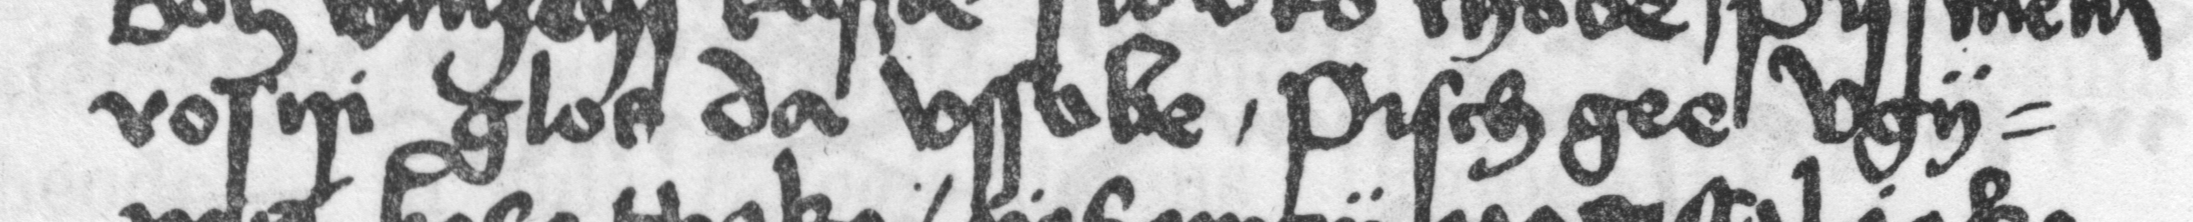
\includegraphics[width=\hsize]{wierszP23}

\splitverse

\parkosz{roſɲi} \parkosz{ġḷos} \parkosz{da} \parkosz{ʋſſobe}/

\indentVerse  \parkosz{Piſch} \parkosz{ġee} \parkosz{\hyphh{Vġij}{ṃo}}

% 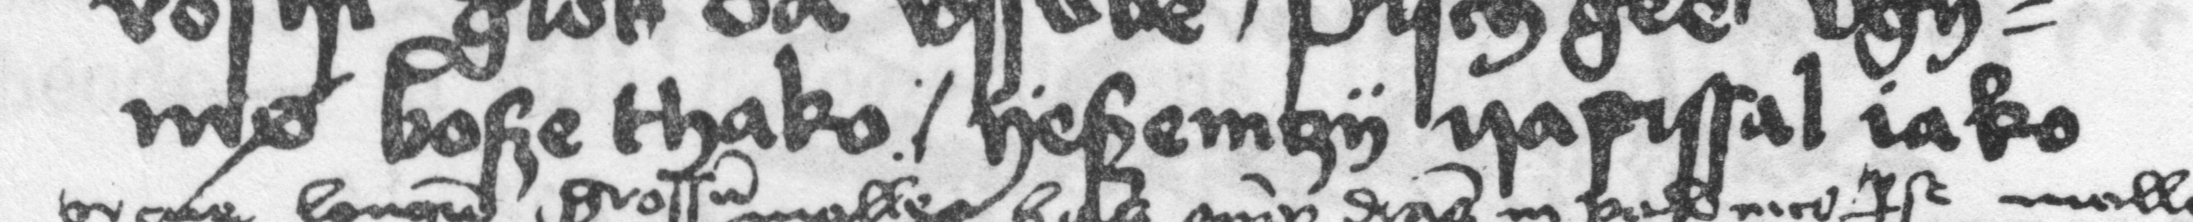
\includegraphics[width=\hsize]{wierszP24}

\splitverse

\parkosz{\hypht{Vġij}{ṃo}} \parkosz{boſze} \parkosz{thako}/

\catcode `\^^M=5
\newtip{86}{Nie sygnalizujemy pisowni w wielu wypadkach niezgodnej z
  zaleceniami. Cały ten wiersz w pisowni zrekonstruowanej według
  wskazówek Parkosza ogłosił Łoś w Języku Polskim I, 1913, s. 56.}
\obeylines
\indentVerse \parkosz{ijeſzeṃczij} \parkosz{ɲapiſſaḷ} \parkosz{iako}¹
% •* Nie sygnalizujemy pisowni w wielu wypadkach niezgodnej z zale¬

% ceniami. Cały ten wiersz w pisowni zrekonstruowanej według wskazówek

% Parkosza ogłosił Łoś w Języku Polskim I, 1913, s. 56.

% koniec wiersza!!!

\newpage

\fulllines

% 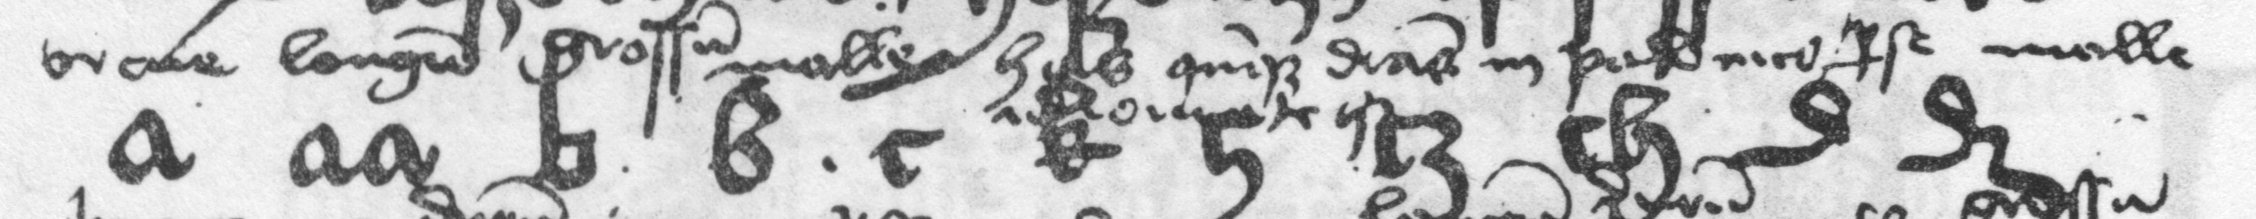
\includegraphics[width=\hsize]{wierszP25-26}


\parkosz{a} breue

\parkosz{aa} longum

\parkosz{ƀ} groſſum

\parkosz{ɓ} molle

c has quinque differencias in Polonico idiomate habet

\parkosz{c} \parkosz{k} \parkosz{ç} \parkosz{cz} \parkosz{ch}

\parkosz{d} per ſe

\parkosz{dz} molle

\parkosz{e} breue

\parkosz{ee} longum

\parkosz{ff} durum

\parkosz{ḟ} molle

% 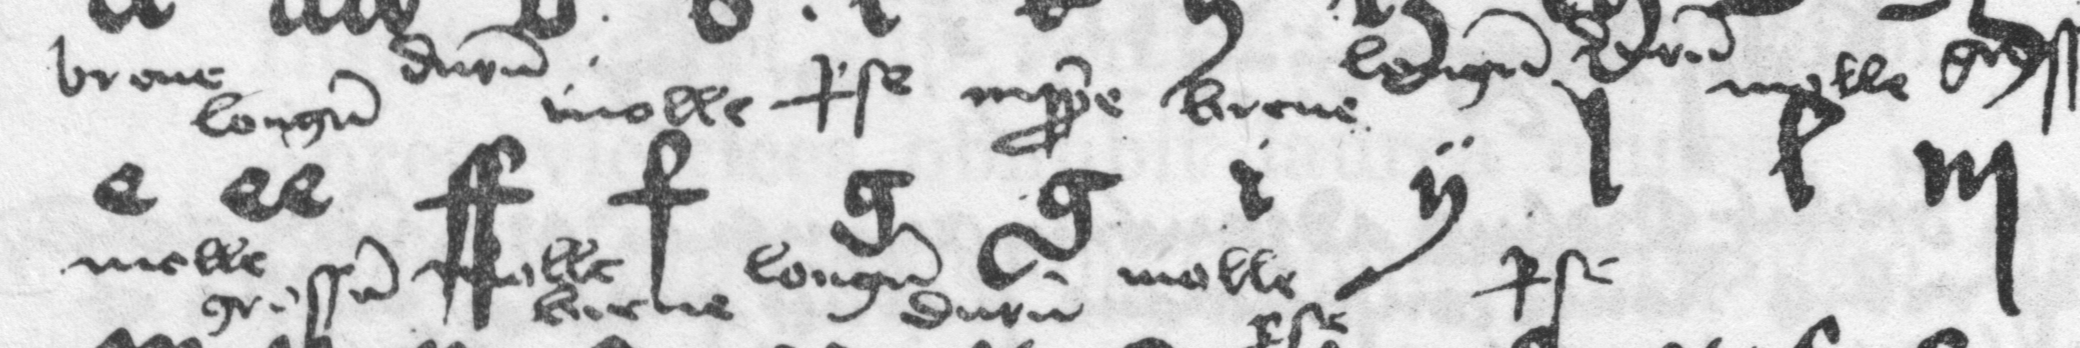
\includegraphics[width=\hsize]{wierszP27-28}



\newtip{87}{Winno być: per se \textit{ꝿ}, improprie \textit{ġ}.}
\parkosz{ġ} per ſe

\parkosz{ꝿ}¹  inproprie
% 87	Winno być: per se g, improprie g.

\parkosz{i} breue

\parkosz{ij} longum

\parkosz{ḷ} durum

\parkosz{ɬ} molle

\parkosz{ɱ} groſſum

\parkosz{ṃ} molle

\parkosz{ɲ}  groſſum

\parkosz{ṇ}   molle

\parkosz{o} breue   

\parkosz{oo} longum

% 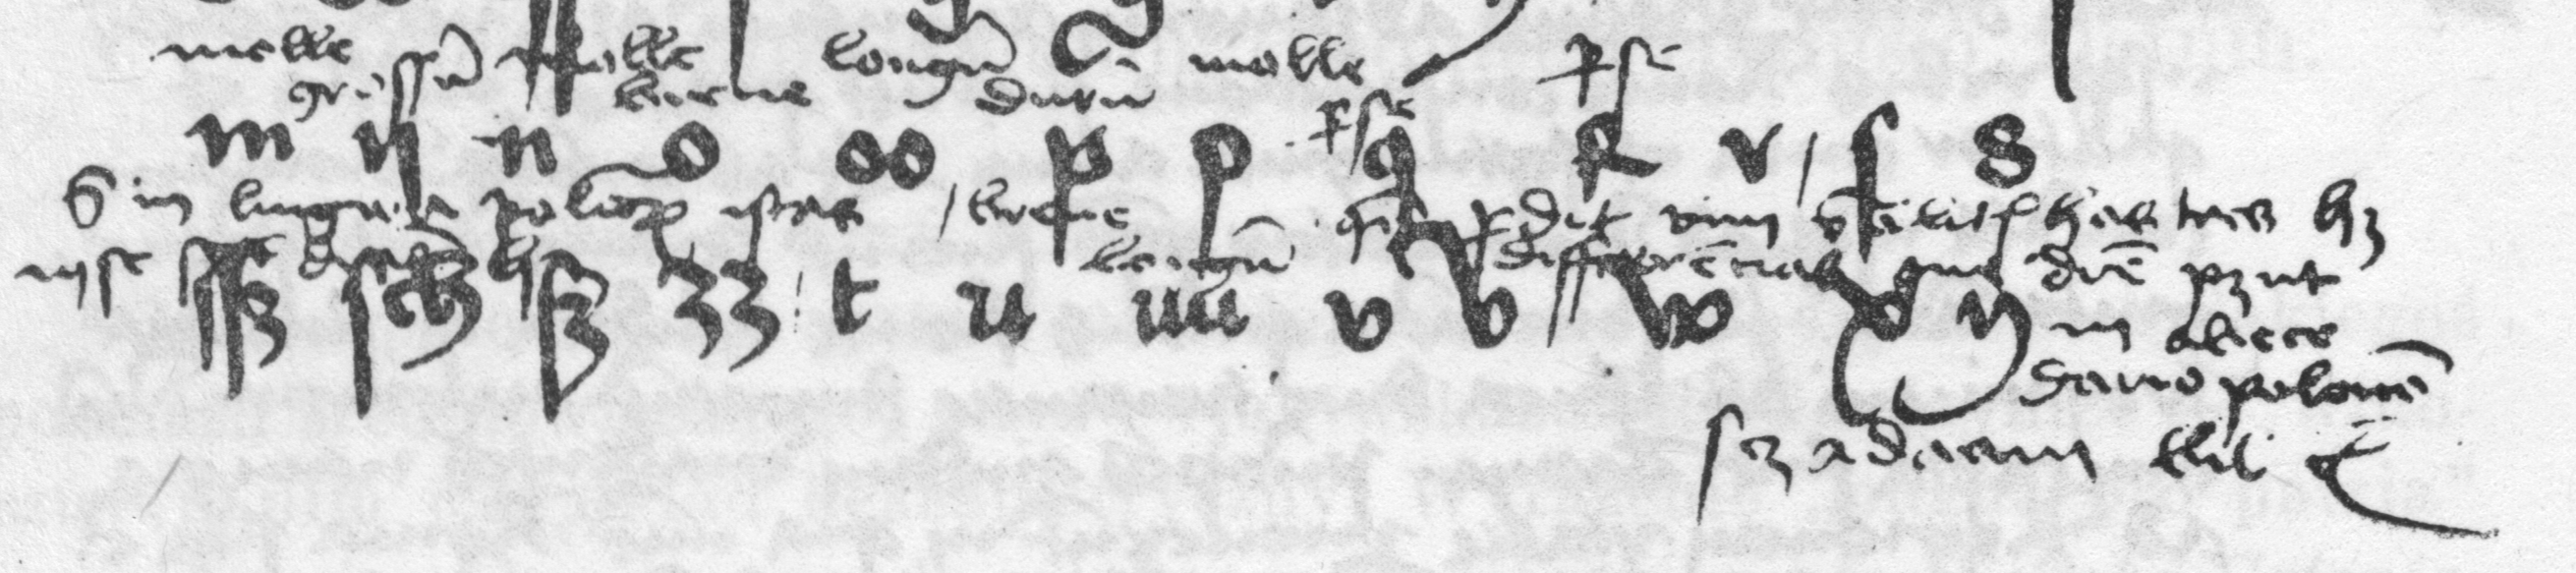
\includegraphics[width=\hsize]{wierszP29-koniec}


\parkosz{ᵽ} durum

\parkosz{ƥ} molle

\parkosz{q} per ſe

\parkosz{R} per ſe

\parkosz{r}

/

\parkosz{S} in lingua Polonorum iſtas in ſe ſex differencias habet       

\parkosz{ſ} \parkosz{s}

\parkosz{ſſz} \parkosz{ſch} \parkosz{ſz} \parkosz{zz}

\parkosz{t}

\parkosz{u} breue	

\parkosz{uu} longum

\parkosz{v} \parkosz{ʋ} \parkosz{w} // \parkosz{x} \parkosz{y}

eum perdit vim vocalitatis, has tres habet differencias,

que differencie patent in abecedario Polonorum,

\parkosz{ſcilicet} \parkosz{adaam} \parkosz{ɓiɬ} etc.  



}

\endinput



% \fullfines

% \ppreviouspageno=16
% \plineno=0


% \fullpreviouslines


% {
% \color{blue}

% ???


% }




% \endinput


%%%%%%%%%%%%%%%%%%%%%%%%%%%%%%%%%%%%%%%%%%%%%%%%%%%%%%%%%%%%%%%%%%%%%%%%%%%%%%%%%%%%%%%%%%%




\catcode `\^^M=5

  \newtip{48}{Łoś niesłusznie uważa, że \textit{bika} w obu wypadkach
    napisano błędnie zamiast \textit{ƀyka}. Przykłady są bowiem podane
    w~pisowni dotychczasowej dla pokazania jej niewystarczalności do
    zróżnicowania wyrazów \textit{bika} i \textit{byka}.}

\obeylines






\newcommand{\margin}[1]{\annotatetextBlue{\{#1\}}{zapisy na marginesie}}


% \renewcommand{\over}[1]{\colorbox{blue!10}{\{#1\}}}

\renewcommand{\over}[1]{\annotatetextBlue{\{#1\}}{zapisy nad rządkami}}

% litery i wyrazy dodane, (których w tekście brak)
%\newcommand{\add}[1]{\colorbox{olive!10}{<#1>}}
\newcommand{\add}[1]{\annotatetextOlive{<#1>}{litery i wyrazy dodane, (których w tekście brak)}}

% litery i wyrazy zbędne
% \newcommand{\extra}[1]{\colorbox{magenta!10}{[#1]}}
\newcommand{\extra}[1]{\colorbox{magenta!10}{[#1]}}

% przekreślenia
% MATHEMATICAL LEFT WHITE SQUARE BRACKET' (U+27E6)
% 'MATHEMATICAL RIGHT WHITE SQUARE BRACKET' (U+27E7)
\newcommand{\overstr}[1]{\annotatetextMagenta{⟦#1⟧}{przekreślenia}}



%%% Local Variables:
%%% mode: latex
%%% TeX-PDF-mode: t
%%% TeX-engine: luatex
%%% TeX-master: "ParkoszLatin"
%%% default-input-method: "Parkosz-slash"
%%% End:
